\documentclass{article}
\usepackage{graphicx}
\usepackage{amsmath}
\usepackage{pgfplots}
\usepackage{siunitx}
\usepackage{cancel}
\usepackage{enumitem}

\newcommand{\mile}{\text{mi}}
\newcommand{\gallon}{\text{gal}}
\newcommand{\kilo}{\text{k}}
\newcommand{\liter}{\text{L}}
\newcommand{\meter}{\text{m}}
\newcommand{\second}{\text{s}}
\newcommand{\foot}{\text{ft}}

\pgfplotsset{compat=1.18}

\usepackage[a4paper, top=1cm, bottom=2cm, left=2cm, right=2cm, includehead, includefoot]{geometry}

\begin{document}

\noindent
Physics 4A - Classical Mechanics \hfill Prof. Roger King

\noindent\rule{\textwidth}{0.4pt}

\begin{center}
    \textbf{\LARGE Homework 1} \\
    \vspace{12pt}
    \large Aaron W. Tarajos \\
    \textit{\today}
\end{center}

\noindent\rule{\textwidth}{0.4pt}

\section*{Problem 1}
The fuel consumption of cars is specified in Europe in terms of liters per 100 km. Convert
30 miles per gallon to this unit. Note that 1 gallon (U.S.) = 3.79 L.

\subsection*{Solution}
We are given \(30 \, \si{\mile\per\gallon}\) and need to convert it to \(\si{\liter\per100\kilo\meter}\). The desired units are the reciprocal of the given units—volume of fuel per distance traveled compared to distance traveled per unit of fuel.

\[
30 \, \frac{\mile}{\gallon} = \frac{1}{30} \, \frac{\gallon}{\mile}
\]
Next, we use chain multiplication to convert miles to kilometers and gallons to liters:

\begin{align*}
\frac{1}{30} \, \frac{\cancel{\gallon}}{\mile} \cdot \frac{3.79 \, \liter}{1 \, \cancel{\gallon}} &= \frac{3.79}{30} \, \frac{\liter}{\mile} \\
\frac{3.79}{30} \, \frac{\liter}{\cancel{\mile}} \cdot \frac{1 \, \mile}{1.609 \, \cancel{\kilo\meter}} &= \frac{3.79}{48.27} \, \frac{\liter}{\kilo\meter} \\
\frac{3.79}{48.27} \, \frac{\liter}{\kilo\meter} &= 0.0785 \, \frac{\liter}{\kilo\meter} = 7.85 \, \frac{\liter}{100 \, \kilo\meter}
\end{align*}

\section*{Problem 2}
Check the following equations for dimensional consistency where \( t \) is time (\si{\second}), \( \nu \) is speed (\si{\meter\per\second}), \( a \) is acceleration (\si{\meter\per\second^2}), and \( x \) is position (\si{\meter}):

\begin{enumerate}
    \item \( x = \frac{\nu^2}{2a} \)
    \item \( x = \frac{1}{2}at \)
    \item \( t = \sqrt{\frac{2x}{a}} \)
\end{enumerate}

\subsection*{Solution}
Checking the dimensional consistency involves verifying that the units balance out correctly on both sides of the equations.

\paragraph{Equation 1: \( x = \frac{\nu^2}{2a} \)}

The units of \( \nu^2 \) and \( 2a \) must cancel such that we are left with just meters (\(\meter\)):

\[
\frac{\left( \meter/\second \right)^2}{\meter/\second^2} = \frac{\meter^2}{\second^2} \cdot \frac{\second^2}{\meter} = \meter
\]
Therefore, Equation 1 is dimensionally consistent.

\paragraph{Equation 2: \( x = \frac{1}{2}at \)}

We are again looking for position in meters (\(\meter\)):

\[
\frac{\meter}{\second^2} \cdot \second \neq \meter
\]
Equation 2 is not dimensionally consistent.

\paragraph{Equation 3: \( t = \sqrt{\frac{2x}{a}} \)}

Here, we are looking for time in seconds (\(\second\)):

\[
\sqrt{\frac{\meter}{\meter/\second^2}} = \sqrt{\second^2} = \second
\]
Equation 3 is dimensionally consistent.

\section*{Problem 3}
A can of paint that covers \(20.0 \, \si{\meter^2}\) costs \$24.60. The walls of a room \(13.0 \, \si{\foot} \times 18.0 \, \si{\foot}\) are \(8.00 \, \si{\foot}\) high. What is the cost of paint for the walls?

\subsection*{Solution}
We need to start by deriving an equation that yields the number of cans of paint required to cover the surface area, $A$, as a function of the given dimensions.
\[
	A = 2h(x_1 + x_2)\ \foot^2
\]
where $x_1$ and $x_2$ are the lengths of the respective edges and $h$ is the height of the walls. If each can is capable of covering $y\ \meter^2$ then then it will cover $3.28084y\ \foot^2$ and so our equation for $n$ cans becomes;
\[
	n = \left\lceil\frac{2h(x_1 + x_2)}{3.28084y}\right\rceil = \left\lceil\frac{2\cdot8.00(13.0 + 18.0)}{3.28084\cdot20}\right\rceil = 3
\]
3 cans at \$24.60 per can gives us a total cost of \$73.80 to paint the walls.

\section*{Problem 4}
Consider a race car on a \(5.00 \, \si{\kilo\meter}\) track. Car A finishes the race in \(4.00 \, \si{\hour}\) and is 1.50 laps ahead of B at this time. What is B's time for the race?

\subsection*{Solution}
We determine Car B's race time by finding how far it has traveled in the time it took Car A to finish the race and then determine the time it would have taken Car B to complete the full distance. Since Car B was \(7.5 \, \si{\kilo\meter}\) behind Car A, Car B traveled \(292.5 \, \si{\kilo\meter}\) in 4 hours. We can then solve for the time \( t_B \) it took Car B to finish the full \(300 \, \si{\kilo\meter}\):

\[
\frac{292.5 \, \si{\kilo\meter}}{4 \, \si{\hour}} = \frac{300 \, \si{\kilo\meter}}{t_B \, \si{\hour}}
\]

\[
t_B = \frac{300 \, \si{\kilo\meter} \cdot 4 \, \si{\hour}}{292.5 \, \si{\kilo\meter}} \approx 4.10 \, \si{\hour}
\]

\section*{Problem 5}
On its maiden voyage in July 1952, the liner \textit{United States} won the coveted Blue Ribbon for
the fastest crossing of the Atlantic from New York to Cornwall, U.K. The trip took 3 days 10
hours 40 min at an average speed of 34.5 knots (65.5 km/h). This was 10 hours 2 minutes less than the
14-year-old record held by the \textit{Queen Mary}. What was the average speed of the \textit{Queen Mary}?

\subsection*{Solution}
The distance across the Atlantic is the same for both ships, so we have:

\[
x = v_1 \cdot t_1 = v_2 \cdot t_2
\]
Solving for \( v_2 \):

\[
v_2 = \frac{v_1 \cdot t_1}{t_2}
\]
Substituting the given values:

\[
v_2 = \frac{65.5 \, \si{\kilo\meter\per\hour} \cdot 82.67 \, \si{\hour}}{92.70 \, \si{\hour}} \approx 58.41 \, \si{\kilo\meter\per\hour}
\]

\section*{Problem 6}
Based on the graph below, estimate the instantaneous velocity at the following times: (a) 1.0 s; (b) 2.5 s; (c) 3.5 s; (d) 4.5 s; (e) 5.0 s;

\begin{figure}[h]
    \centering
    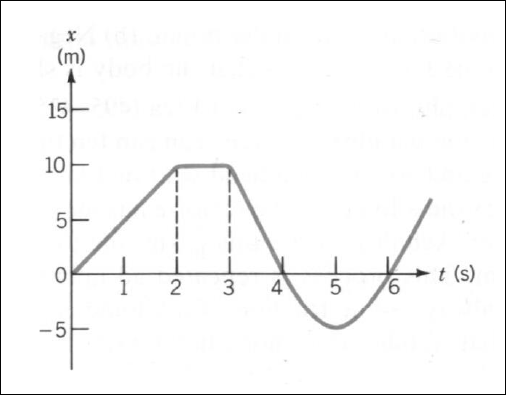
\includegraphics[scale=0.5]{graph.png}
    \label{fig:my_graph}
\end{figure}

\subsection*{Solution}

\begin{enumerate}[label=(\alph*)]
    \item \(5 \, \si{\meter\per\second}\)
    \item \(0 \, \si{\meter\per\second}\)
    \item \(-10 \, \si{\meter\per\second}\)
    \item \(-3 \, \si{\meter\per\second}\)
    \item \(0 \, \si{\meter\per\second}\)
\end{enumerate}

\section*{Problem 7}
At \( t = 2.25 \, \si{\second} \), a particle is at \( x = 7.00 \, \si{\meter} \) and has velocity \( v = 3.50 \, \si{\meter\per\second} \). At \( t = 7.00 \, \si{\second} \), it is at \( x = -5.10 \, \si{\meter} \) and has velocity \( v = 6.00 \, \si{\meter\per\second} \). Find: (a) its average velocity; (b) its average acceleration.

\subsection*{Solution}
The average velocity is defined as:

\[
v_{\text{avg}} = \frac{\Delta x}{\Delta t} = \frac{x_2 - x_1}{t_2 - t_1}
\]
Substituting the values:

\[
v_{\text{avg}} = \frac{-5.10 \, \si{\meter} - 7.00 \, \si{\meter}}{7.00 \, \si{\second} - 2.25 \, \si{\second}} = \frac{-12.10 \, \si{\meter}}{4.75 \, \si{\second}} \approx -2.55 \, \si{\meter\per\second}
\]
The average acceleration is defined as:

\[
a_{\text{avg}} = \frac{\Delta v}{\Delta t} = \frac{v_2 - v_1}{t_2 - t_1}
\]
Substituting the values:

\[
a_{\text{avg}} = \frac{6.00 \, \si{\meter\per\second} - 3.50 \, \si{\meter\per\second}}{7.00 \, \si{\second} - 2.25 \, \si{\second}} = \frac{2.50 \, \si{\meter\per\second}}{4.75 \, \si{\second}} \approx 0.53 \, \si{\meter\per\second^2}
\]

\section*{Problem 8}
The position of a particle is given by \( x = 4.50e^{-0.30t} \), where \( x \) has units of meters. What is (a) the average velocity between 2.00 and 3.00 s; (b) the instantaneous velocity at 2.00 s; (c) the instantaneous acceleration at 2.00 s.

\subsection*{Solution}
\subsubsection*{Part a}
The average velocity is the change in position over the change in time. First, find the positions at \( t = 2.00 \, \si{\second} \) and \( t = 3.00 \, \si{\second} \):

\[
x(3) = 4.50e^{-0.9}, \quad x(2) = 4.50e^{-0.6}
\]
The average velocity is then:

\[
v_{\text{avg}} = \frac{4.50e^{-0.9} - 4.50e^{-0.6}}{3 - 2} \approx -0.64 \, \si{\meter\per\second}
\]

\subsubsection*{Part b}
The instantaneous velocity is the derivative of the position function:

\begin{align*}
v(t) &= \frac{d}{dt} \left( 4.50e^{-0.30t} \right) \\
&= -0.30 \cdot 4.50e^{-0.30t} \\
&= -1.35e^{-0.30t}
\end{align*}
Evaluating at \( t = 2.00 \, \si{\second} \):

\[
v(2) = -1.35e^{-0.6} \approx -0.74 \, \si{\meter\per\second}
\]

\subsubsection*{Part c}
The instantaneous acceleration is the derivative of the velocity function:

\[
a(t) = \frac{d}{dt} \left( -1.35e^{-0.30t} \right) = 0.405e^{-0.30t}
\]
Evaluating at \( t = 2.00 \, \si{\second} \):

\[
a(2) = 0.405e^{-0.6} \approx 0.25 \, \si{\meter\per\second^2}
\]

\end{document}
